\chapter{Evaluation}
This chapter shows the results of the experiments and how the gathered data can be interpreted. 

\subsection{output format}
Figure \ref{entries} shows the format of a single entry after the decryption. 

\begin{figure}[!htb]
\centering
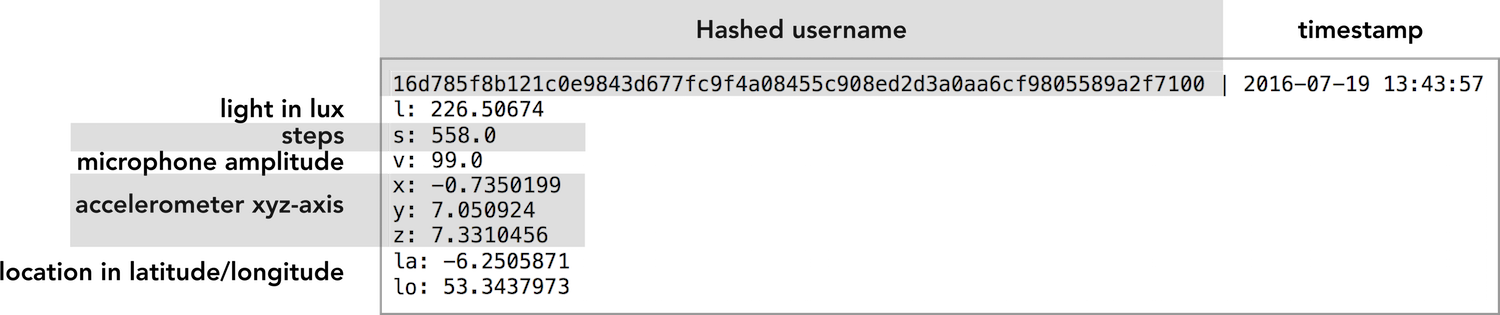
\includegraphics[width=\textwidth]{entries}
\caption{gathered data}\label{entries}
\vspace{10 mm}
\end{figure}

\FloatBarrier

\section{Crowd Experiment}
This section shows the finding in the experiment where the participants had to solve the programming task. This section is divided into the different categories where the findings were clustered into. 

\subsection{Noise}
Regular phone microphones are not calibrated to provide an general loudness. Therefore we can use the values of the environmental noise only for finding peeks or changes.
The environmental noise shows a steady low noise level for four of the participants while one participant has some high peeks in the data. 

\subsection{Dynamic in Light and Noise}
\FloatBarrier

\begin{table}[ht]
  \begin{tabular}{|P{3cm}|P{1.6cm}|P{1.6cm}|P{1.6cm}|P{1.6cm}|P{1.6cm}|}
   	\textbf{Noise}				& \textbf{P1}			& \textbf{P2}			& 	\textbf{P3}		& 	\textbf{P4}			& 	\textbf{P5}	\\ \hline
  	Dynamic Score				& 139.72					& 78.51					& 37.61				& 67.80					& 59.63			\\ \hline
  	Average 						& 1,676.59				& 549.59					& 159.82				& 1033.95				& 498.67			\\ \hline
  	\end{tabular}
  	\newline\newline
  	\caption{Dynamic Noise Level}\label{dynNoise}
\end{table}

\begin{table}[ht]
  \begin{tabular}{|P{3cm}|P{1.6cm}|P{1.6cm}|P{1.6cm}|P{1.6cm}|P{1.6cm}|}
   	\textbf{Light}				& \textbf{P1}			& \textbf{P2}			& 	\textbf{P3}		& 	\textbf{P4}			& 	\textbf{P5}	\\ \hline
  	Dynamic Score				& 2.46						& 2.44						& 	-						& 12.73					& 0.26				\\ \hline
  	Average 						& 7.37						& 5.69						& 	-						& 59.73					& 1.35				\\ \hline
  	\end{tabular}
  	\newline\newline
  	\caption{Dynamic Light Level}\label{dynLight}
\end{table}

The standard deviation added and subtracted from the mean is the range that separates normal noise and peeks. The values are only in a positive range. If the minimum value goes negative in the calculation it was set to zero instead. 
The values outside of the range as a percentage relatively to the standard deviation were added together and result in a number which can give a good indicator of the amount and level of dynamic. 
These value divided by the number of minutes of the gathering create the dynamic score which indicates the level of dynamic in a dataset.
The average value is the mean of all the percentage values outside of the range.

\FloatBarrier

\subsection{Location}
The location of the participants was not gathered from two participants. Two of the other participants were working in Dublin, Ireland while a third one did the task in Madrid, Spain.\\
The step counter of the participants didn't provide valuable information as the step count was never more than 10 and didn't change during the gathering process. Also the location of the participants didn't change during the experiment. Thus, we can assume that the participants didn't move during the experiment.

\subsection{Movement}
The 3-axis accelerometer of the participants devices don't show any changes. In all the gathered results, the device was laying on the desk without big movements in between. A value close to 0 for the X and Z axis of the measurements as well as a value close to 10 for the Z axis show that the mobile phones were positioned screen upwards on a horizontal surface. Any movements of the device would have changed at least one of the values of an axis. 

\subsection{Weather}
\FloatBarrier

\begin{table}[ht]
  \begin{tabular}{|P{3cm}|P{3cm}|P{3cm}|P{3cm}|}
   \textbf{Description}		& \textbf{Temperature}		& \textbf{Humidity}		& 	\textbf{Pressure}		\\ \hline
   	- 									& -										& -								& -								\\ \hline		%p1
   	Cloudy and Drizzly 		& 17\degree C						& 	82\%						& 1007 nPA					\\ \hline		%p2
   	 - 									& -										& -								& -								\\ \hline		%p3
   	Sunny 							& 31\degree C						& 	31\%						& 1018 nPA					\\ \hline		%p4 
   	Cloudy 							& 14\degree C						& 	62\%						& 1028 nPA					\\ \hline		%p5
  \end{tabular}
  \newline\newline
  \caption{Weather during experiment}\label{weather}
\end{table}

The weather is looked up based on the location, data and time. Therefore, the weather of the two participants without location was not possible to find out. The weather of the experiments of two participants was cloudy for one, and cloudy with a little bit of rain for the other one. The third participants had a hot sunny day. The individual information can be seen in table \ref{weather}.
\FloatBarrier

\subsection{Light and Environment}
The results \ref{ligps} show a good probability that all the participants where working on the task indoor. Based on the classification mentioned in the previous section, the highest brightness of the participants environment with 554.33 lux, which is a in the section of a office space or a very dark day \ref{inLight} \ref{outLight}. However, the mentioned maximum value is a peek in the results of a single participant. Another participant whose light level was on a high level was working during a sunny time which removes the possibility that it was a very dark day and that the participants was working outside. 
The other two participants had a lower light measured and therefore just a small possibility that they were actually working outside.  
Also the location of the participants are all in urban areas within a range of several buildings. 

\subsection{Development Performance}
The performance in software development is not only measured by the quality of the resulting code also the actual efficiency of the programmer matters especially for companies.
The code from the experiment is analyzed based on these three aspects.  

\begin{table}[ht]
  \begin{tabular}{|P{2.5cm}|P{1.8cm}|P{1.8cm}|P{1.8cm}|P{1.8cm}|P{1.8cm}|}
   	\textbf{Light}				& \textbf{P1}			& \textbf{P2}			& 	\textbf{P3}		& 	\textbf{P4}			& 	\textbf{P5}			\\ \hline
  	Src code lines per min	& 5.74						& 5.12						& 	1.16					& 0.58						& 0.36						\\ \hline
  	lines of src Code 			& 69							& 95							& 	20					& 35							& 33							\\ \hline
  	max nesting depths		& 1							& 3							& 	2						& 2							& 2							\\ \hline
  	unnecessary lines			& 0							& 0							& 	2						& 5							& 0							\\ \hline
  	no intending					& 0							& 0							& 	0						& 0							& 0							\\ \hline
  	duplicated code			& 0\%						& 0\%						&	 0\%					& 0\%						& 0\%						\\ \hline
  	\end{tabular}
  	\newline\newline
  	\caption{Code Performance}\label{codePerformance}
\end{table}

A tool named "Teamscale" was used for the code analysis. The systems analysis the code for Structure Metrics like lines of code, nesting depth etc. It also detects comments, test coverage, architecture conformance, code duplications and Anomalies like naming convention violations \cite{heinemann2014teamscale}.
\bigbreak
The limited size of the project from the experiment also provides only limited code analysis information. However, to actually rank the code and it's quality, the following categories were used to calculate an actual quality score. 
The different quality factor either decrease or increase the score of the code depending weather its  negative or positive factor. The lowest score at the end signals the best code. 
Testing the code was not part of the experiment and therefore a factor which can't take any influence in the results. 

\subsubsection{Efficiency}
The efficiency of the code is calculated by the productivity by written source code lines per minutes. The more code the developer wrote per minute, the more productive he/she is. 
The lines of code of the project are in indicator of the complexity of the solution. Solving the same problem with less code is mostly a sign that the developer reduced the complexity and created better code. 
Also the nesting depth within the code is a factor in the efficiency of solving a problem. The deeper the nested loops are, the more complex it gets. In the majority it is better to keep the nested depth as low as possible. 
The longest method length was not used as an indicator because long method names can be more descriptive as well as too confusing. Therefore it can't be detected only from the metrics if it's positive or negative. 

\subsubsection{Code Quality}
Having single lines of white-space is alright to keep the structure of the code clean but several lines are just reducing the code that a developer can see on the screen and should be avoided. 
In this section also the formatting is been looked at. Code without indented code blocks is massively decreasing the readability of the code and makes it very hard to get an overview. 

It is also a bad habit to have duplicated code at different places in the project. That reduces the maintainability and can cause bugs or unexpected behavior. Here, the amount of duplicated code is shown in percentage. Luckily, none of the participants had any duplications in the code. 

\subsection{Variable and Method/Function Naming}
The naming of the variables is detected by hand. A script can extract the variable names and method names of a project to make it easier for a large code base and multiple projects. For this experiment, we just looked at meaningful names rather than abbreviations which meaning can just be guessed. 
The evaluation of the naming of variables and methods should be descriptive and help others to understand the code. The code of the participants is not showing a very good example neither shows it a very bad one. Participant 4 was using the best naming for the variables while the method names are not clear. The best naming for methods can be found in the code of participant number 2. 
The least descriptive variable naming was done by participant 5 and the method name of participant of participant 4 where confusing in the functionality of the methods.

\subsection{Coding Conventions}
Coding conventions such as using camelCase for variables and method names starting lowercase and Class names starting Uppercase are some examples for coding conventions that should not be changed within a project to help to increase readability. 
The above mentioned conventions as well as keeping a constant style was followed by all participants except of participant number 5, who was switching between camelCase and underscore for variable names. 

\subsection{Results}
The experiment demonstrates that the application for collecting data works well and creates valuable data that can be used to to find evidence for influencing factors in development quality when it will be applied in a larger scope. 
\\bigbreak
The evaluation of the data showed that different results in the developing quality always had more than just one factors that are differentiating the work and environmental patterns \ref{codePerformance}. Also, the quality software developing is assembled from different components and can't be used as a general term.
\bigbreak
Participant 4 was the only participants who stated to be distracted during the experiment results show that there could be a possible correlation between the dynamic changes in the light level of the distraction as this participant has by far the highest dynamic score and highest average in the relative amplitude \ref{dynLight}.
The noise didn't show clear evidence as the results in the coding task don't show a pattern for the two highest values of participant 1 and participant 4. 
Also no evidence was found that the solving time of the experiments has any influence in the length and quality of the code.
Correlations between weather and any code metrics were not found within the results.  

\FloatBarrier

\subsection{Problems}
The gathering process showed some problems with the permissions of different mobile devices and different settings. Not every device has the same sensors and some devices have different default security settings that permit to access specific data within the application even when the application itself has permissions granted. Furthermore the usage of different programming languages for the experiments made it difficult to compare the results with each other. 
A larger group as well as a larger project with more resulting source code was not achievable in the scope of this dissertation but mandatory to detect influences rather than just plausible factors.
\\
At the first place, the idea was to let the participants do the task whenever they want to find out whether they work at night or day. However, it turned out that the majority of the participants confirmed to do it but actually forget it all the time and at the end did it right after a being reminded. So, the time of the day can not be used as a indicator for detecting the working times of participants. 

\section{Individual Experiment Results}
The results of the individual experiment are demonstrating the usage and the abilities for the Dather Application for a single participant. Rather than in the first experiment, it is taking only the data of a single person into account.
The data only shows a plausible factor but doesn't confirm the influences of the tested factors. A lot more test cases would be needed to create a more accurate average value. However, the purpose of this experiment was to demonstrate the usage of the data in more controlled comparable environments rather than in the other experiment which detected the environment and patterns. 
\bigbreak
The graphs of the three scenarios \ref{coffeeGraph}, \ref{musicGraph} and \ref{runGraph} shows an overview of the durations, the participant needed to solve the Sudokus. The black dots are signaling the solving time on the y-axis for each of the ten measurements per scenario. The horizontal line in every scenario is at the position of average during, the participant needed to solve the Sudokus. 

\FloatBarrier
\subsection{Coffee}
The the scatter plot \ref{coffeeGraph} shows the times of 10 Sudoku solvings of the participant. The exact time can be seen in table \ref{coffee} in the appendix.
\bigbreak
The results shows an average time which the participant needed without drinking coffee was \textbf{14:24 minutes} and after consuming \textbf{17:37 minutes} minutes per Sudoku. The participant needed 3:13 minutes or 22.34\%  longer after having a strong coffee.\\
These results are different than the findings in \cite{liguori1997absorption}, who found that a similar amount of caffeine (400 mg) increases the cognitive performance. \\
However, in our case the participant of the Experiment mentioned to feel fretful after the intake of the high amount of caffeine. That could be a reason for the lower performance of the subject. Thus, it is possible that a overdose had negative impact on the participant and lower amount of caffeine would have had resulted better. 

\begin{figure}
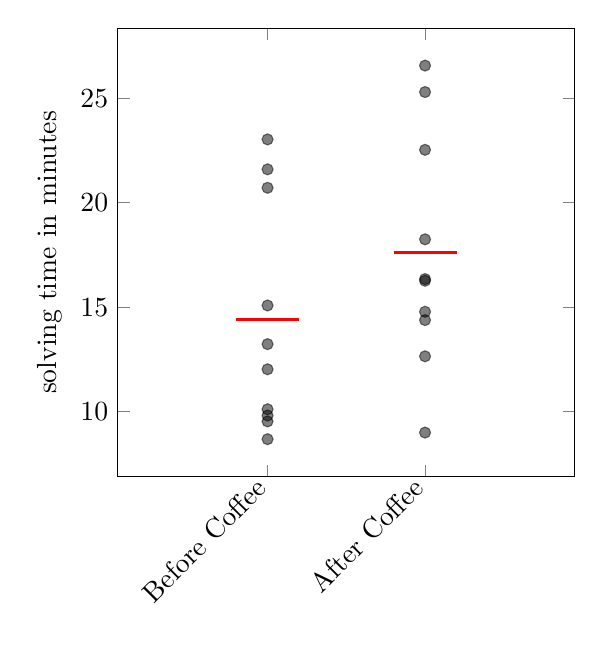
\begin{tikzpicture}
\begin{axis}[
ylabel=solving time in minutes,
xtick={0,1},
xticklabels={Before Coffee, After Coffee},
x=2cm,
x tick label style={rotate=45, anchor=east, align=center},
enlarge x limits={abs=1.5cm}, 
scatter/classes={%
    a={mark=*,draw=black}}]
\addplot[scatter,only marks, fill opacity=0.5, opacity=0.5, 
    scatter src=explicit symbolic]
table[meta=label] {
x 	y 						label
0	20.716667		1
0	21.6					2
0	13.233333		3
0	23.0333333	4
0	9.533333		5
0	12.03				6
0	15.0833333	7
0	9.816667		8
0	10.116667		9
0	8.683333		10
};

\addplot[mark=none, color=red, very thick] 
coordinates {
(-0.2, 14.42) 
(	0.2,14.42)
};

\addplot[scatter,only marks, fill opacity=0.5, opacity=0.5,
    scatter src=explicit symbolic]
table[meta=label] {
x 	y	 				label
1 12.65			1
1 22.533333	2
1 9.0				3
1 26.566667	4
1 14.383333	5
1 16.35			6
1 25.3				7
1 16.266667	8
1 14.783333	9
1 18.25			10
};

\addplot[mark=none, color=red, very thick] 
coordinates {
(0.8, 17.62) 
(	1.2,17.62)
};

\end{axis}
\end{tikzpicture}
\caption{Scatter Plot: Coffee} \label{coffeeGraph}
\end{figure}

\FloatBarrier

\subsection{Music}

\ref{musicGraph} and \ref{music} show the times of the Sudokus that have been solved by the participant and the duration it took. It shows that the average time of solving was the shortest when the participant was listening to music. 
The participant solved the ten Sudokus in 89.35\% of the average time compared to the results archived without music. That is \textbf{1 minute and 34 seconds less time in average}. 
On the other hand, the average solving time while listening to heavy metal music was 4.08 \% or 36 seconds slower than without listening to music. 
The results show evidence that for the participant the cognitive performance in solving Sudoku riddles was increasing when listening to classical music and decreasing at heavy metal music. 

\FloatBarrier

\begin{figure}
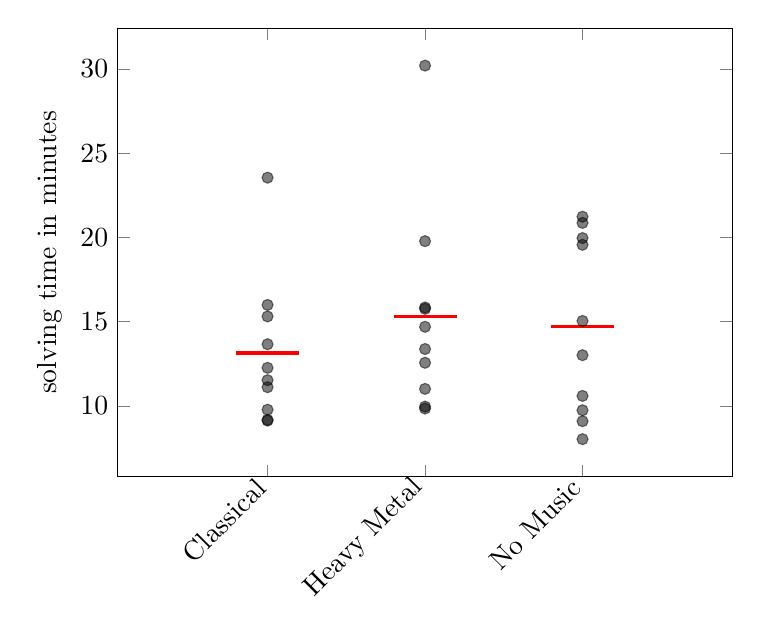
\begin{tikzpicture}
\begin{axis}[
ylabel=solving time in minutes,
xtick={0,1,2},
xticklabels={Classical, Heavy Metal, No Music},
x=2cm,
x tick label style={rotate=45, anchor=east, align=center},
enlarge x limits={abs=1.5cm}, 
scatter/classes={%
    a={mark=*,draw=black}}]
\addplot[scatter,only marks, fill opacity=0.5, opacity=0.5, 
    scatter src=explicit symbolic]
table[meta=label] {
x 	y 						label
0	13.666667		1
0	12.266667		2
0	9.183333		3
0	11.116667		4
0	15.316667		5
0	9.783333		6
0	11.533333		7
0	9.133333		8
0	16.0					9
0	23.55				10
};

\addplot[mark=none, color=red, very thick] 
coordinates {
(-0.2, 13.15) 
(0.2, 13.15)
};

\addplot[scatter,only marks, fill opacity=0.5, opacity=0.5,
    scatter src=explicit symbolic]
table[meta=label] {
x 	y	 					label
1	30.2					1
1 	15.85				2
1 	14.7					3
1 	15.766667		4
1 	19.783333		5
1 	9.85					6
1 	11.0166667	7
1 	12.566667		8
1 	9.966667		9
1 	13.383333		10
};

\addplot[mark=none, color=red, very thick] 
coordinates {
(0.8, 15.316667) 
(	1.2,15.316667)
};

\addplot[scatter,only marks, fill opacity=0.5, opacity=0.5,
    scatter src=explicit symbolic]
table[meta=label] {
x 	y	 					label
2 	20.866667		1
2 	9.75					2
2 	21.233333		3
2 	13.0166667	4
2 	9.1					5	
2 	19.566667		6
2 	8.0333333		7
2 	10.6					8
2 	19.966667		9
2 	15.05				10
};

\addplot[mark=none, color=red, very thick] 
coordinates {
(1.8, 14.716667) 
(	2.2,14.716667)
};

\end{axis}
\end{tikzpicture}
\caption{Scatter Plot: Music} \label{musicGraph}
\end{figure}


\FloatBarrier

\subsection{Running}
The graph \ref{runGraph} results show a trend for a better performance after strong physical activity. Table table with the exact times can also be found in the appendix \ref{running}.The average solving time after the run (\textbf{10:52 min}) is 3:20 min faster than the \textbf{14:12} minutes before running. That is a decrease of \textbf{22.5\%} from before to after and can be seen in \ref{resultRunning}. 
Compared to the two other individual experiments, the results of this scenario are differing more at each measurement. 4 times, the solving after the running took actually longer than the completion in the pre-run state. 

\begin{figure}
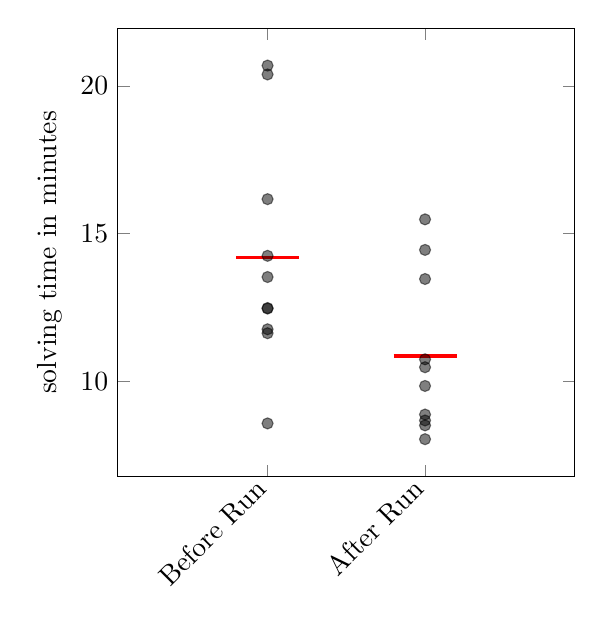
\begin{tikzpicture}
\begin{axis}[
ylabel=solving time in minutes,
xtick={0,1},
xticklabels={Before Run, After Run},
x=2cm,
x tick label style={rotate=45, anchor=east, align=center},
enlarge x limits={abs=1.5cm}, 
scatter/classes={%
    a={mark=*,draw=black}}]
\addplot[scatter,only marks, fill opacity=0.5, opacity=0.5, 
    scatter src=explicit symbolic]
table[meta=label] {
x 	y 						label
0	12.466667		1
0	11.633333		2
0	12.483333		3
0	20.383333		4
0	8.583333		5
0	16.166667		6
0	14.25				7
0	11.766667		8
0	13.533333		9
0	20.683333		10
};

\addplot[mark=none, color=red, very thick] 
coordinates {
(-0.2, 14.2) 
(0.2, 14.2)
};

\addplot[scatter,only marks, fill opacity=0.5, opacity=0.5,
    scatter src=explicit symbolic]
table[meta=label] {
x 	y	 				label
1 	14.45			1
1 	10.483333	2
1 	15.483333	3
1 	8.05				4
1 	8.883333	5
1 	9.85				6
1 	10.75			7
1 	13.466667	8
1 	8.683333	9
1 	8.516667	10
};

\addplot[mark=none, color=red, very thick] 
coordinates {
(0.8, 10.866667) 
(1.2, 10.866667)
};

\end{axis}
\end{tikzpicture}
\caption{Scatter Plot: Running} \label{runGraph}
\end{figure}


\FloatBarrier
